\documentclass{article}
\usepackage{a4wide}
\usepackage{norsk}
\usepackage{amsmath}
\usepackage{amssymb}
\usepackage{dsfont}
%\usepackage[dvips]{epsfig}
%\usepackage{graphicx}
\usepackage{fancyhdr}
\usepackage{listings}
\usepackage{nomencl}
\usepackage[pdftex]{graphicx}

\pagestyle{fancy}
\lhead{\footnotesize \parbox{11cm}{Andreas Johann H\"ormer (753179)}}
\rhead{\footnotesize {Laboratory 1}}
\chead{\footnotesize {TTT4170}}

\title{Report Room acoustics (Lab 1)}
\author{Andreas Johann H\"ormer}
\date{14.02.2014}

\begin{document}
\thispagestyle{empty}
\maketitle
\thispagestyle{empty}
%\\[5cm]
\begin{center}
TTT4170 Audio Technology\\[3cm]
Lab group:
\begin{itemize}
\item Andreas Johann H\"ormer
\item Milan Stojkovic
\item y\\[3cm]
\end{itemize}
Report delivered: 27.02.2014\\[6cm]
FACULTY OF INFORMATION TECHNOLOGY, MATHEMATICS AND ELECTRICAL ENGINEERING\\
NORWEGIAN UNIVERSITY OF SCIENCE AND TECHNOLOGY
\end{center}
\thispagestyle{empty}
\tableofcontents
\thispagestyle{empty}
\newpage
\section*{Summary}
\thispagestyle{empty}
This report regards to the first laboratory exercise of Audio Technology at NTNU. It covers measurements and calculations with subject to room acoustics.\\
The reverbation time of a lecture room\footnote{EL2, Elbygget 1st floor, Gloshaugen Campus of NTNU} was measured. The reverbation time was measured at three positions, one in the front, in the middle and in the back of the room. Duration of reverb is about 0.7s from 500Hz to 4kHz and decreasing after this. At low frequency ranges there are some interesting results and huge variations in reverbation time. This is because of large wavelength $\lambda$.\\
Sound pressure level (SPL) was measured in a straight line from the sound source to the back of the room. The result shows that until the hall radius is reached the SPL degrades quickly and remains at lower slope after the hall radius. This is because of significant influence of reverbation effects.\\
An average calculation factor for every octave band has been calculated, as well as an option for decreasing the reverbation time to 0.5s. A hall radius is calculate, which is at a distance of 1.33m from the sound source. In the measurements it has been shown, that the real hall radius is a little bit farer away than the calculated one, because of assumed omnidirectionality of the loudspeaker.
\newpage
\setcounter{page}{1}
\section{Introduction}
This laboratory exercises treated different measurement and calculation methods of room acoustics. Therefore the dimensions of a room are measured and reverbation times at different octave bands and sound pressure levels as function of distance to the sound source are calculated. Sabine's formula is used for calculations. Further the hall radius in the room and absorption coefficients at different frequency bands are calculated.\\
Measurements were done in the lecture room EL2 in Elbygget of NTNU. The dimensions of the room were measured with a BOSCH laser meter and rounded to the next meter. The room is 10m width and 10m long, the ceiling is 4m in the front and 3m in the back. The floor is 3.4m horizontal and has a slope starting at 3.4m to the end at 10m. A shape of the auditorium can be seen in figure \ref{fig:shape}. The floor is linoleum, at the slope there are chairs. On the backside there are some absorbers, the left side is gypsum, at the right side of the lecture hall are mostly glass areas (windows). In the front there is a wooden blackboard at the wall, the ceiling is gypsum. EL2 has a volume of $V=367m^3$ and a surface area of $S=344m^2$. The calculation can be found in chapter \ref{sec:roomparam}.
\begin{figure}[htbp]
\begin{center}
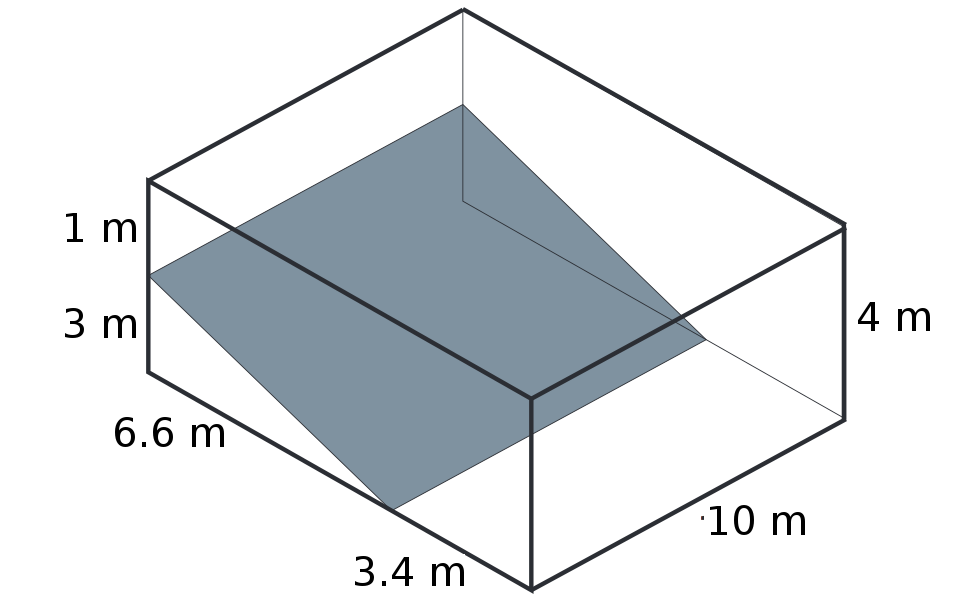
\includegraphics[width=8cm,keepaspectratio=true]{roomshape}
\caption{Shape of auditorium EL2}
\label{fig:shape}
\end{center}
\end{figure}
\section{Theory}
\subsection{Room reverbation}
In figure \ref{fig:irtheory} a typical room reverbation is shown. After a strong direct sound early reflections occur, which can be seperated very clearly. After some time the reflections are smoothed and different reverbation peaks cannot been seperated. Then late reflections occur. 
\begin{figure}[htbp]
\begin{center}
\includegraphics[width=8cm,keepaspectratio=true]{ir}
\caption{Impulse response with early reflections and reverbation}
\label{fig:irtheory}
\end{center}
\end{figure}

\subsection{Formulary}
\subsubsection{Room parameters}
In this section some formulary for calculations are mentioned. These formulas are helpful for calculating room acoustical parameters.
Some equations to get room parameters like volume and surface area are
\begin{equation}
V_{room,total}=V_{room}-V_{under\ shaped\ area}
\end{equation}
with
\begin{equation}
V=l\cdot h\cdot w
\end{equation}
and
\begin{equation}
S_{total}=S_{front}+2\cdot S_{side}+S_{back}-2\cdot S_{side\ below\ slope}+S_{ceiling}+S_{floor}+S_{slope}
\end{equation}
\subsubsection{Acoustical parameters}
\begin{equation}
\alpha=\frac{0.161\cdot V}{T_{60}\cdot S}
\end{equation}
\begin{equation}
T_{60}=\frac{k\cdot V}{A}=\frac{0.161\cdot V}{\alpha\cdot S}
\end{equation}


The hall radius can be calculated using
\begin{equation}
r_H=\sqrt{\frac{V}{100\cdot\pi\cdot T_{60}}}
\end{equation}

\begin{equation}
\bar{\alpha}=\frac{\alpha_1\cdot S_1+\alpha_2\cdot S_2}{S_1+S_2}
\end{equation}

For a more accurate calculation Eyring's formula can be used. In this formula the frequency and air parameters like speed of sound and air humidity are taken into account. 
\begin{equation}
A=S\cdot\bar{\alpha}+4\cdot m\cdot V
\end{equation}
\begin{equation}
m\approx\frac{0.074}{\Phi}\cdot f^2
\end{equation}
where
\begin{itemize}
\item $\Phi$ is the relative humidity
\item $f$ is frequency in kHz
\end{itemize}
\begin{equation}
\bar{\alpha}=\frac{0.161\cdot V-(S-S_{grey})\cdot\alpha-4\cdot m\cdot V}{S_{grey}}
\end{equation}
\section{Measurements}
\subsection{Equipment}
The measurements were done with a notebook and WinLMS-Software. A measurement microphone was put on a microphone stand. As sound source a loudspeaker (which is assumed as omnidirectional) was used.
\subsection{Reverbation time}
\subsubsection{Method}
For measuring the reverbation time of the room the microphone was placed at three different positions. One was chosen in the back of the room, one in the middle and one in a corner in the front. The exact positions in the lecture room can be found in table \ref{tab:revmeasure}. The measurements were done with a swept sine with starting frequency 50Hz to an end frequency of 20kHz. This is done in every measurement point, then the results are averaged.
\begin{table}
\begin{center}
\begin{tabular}{|c c|}
\hline
\includegraphics[width=6cm,keepaspectratio=true]{frontpic} & 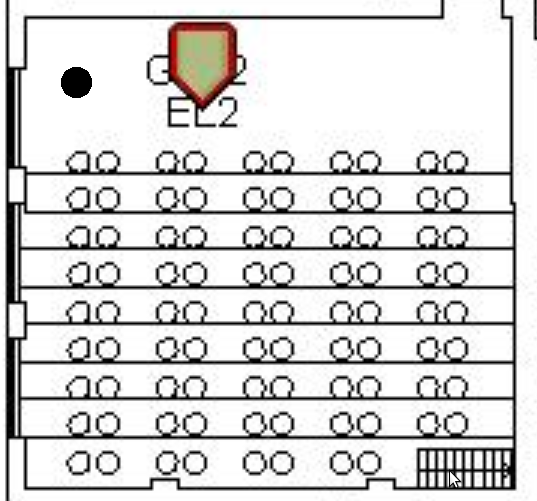
\includegraphics[width=5cm,keepaspectratio=true]{front}\\
\multicolumn{2}{|c|}{measurement in the left front corner}\\
\hline
\includegraphics[width=6cm,keepaspectratio=true]{middlepic} & 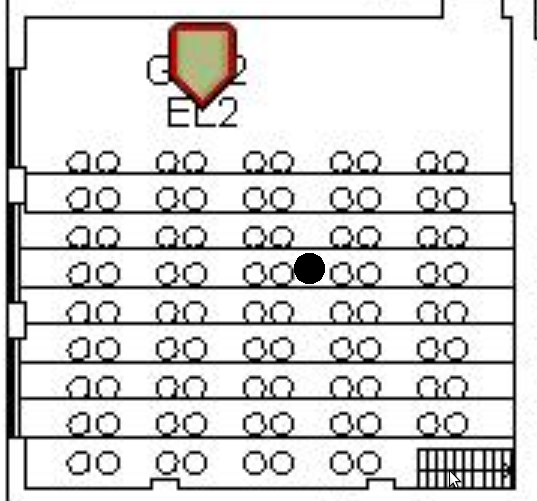
\includegraphics[width=5cm,keepaspectratio=true]{middle}\\
\multicolumn{2}{|c|}{measurement in the middle of the room}\\
\hline
\includegraphics[width=6cm,keepaspectratio=true]{backpic} & 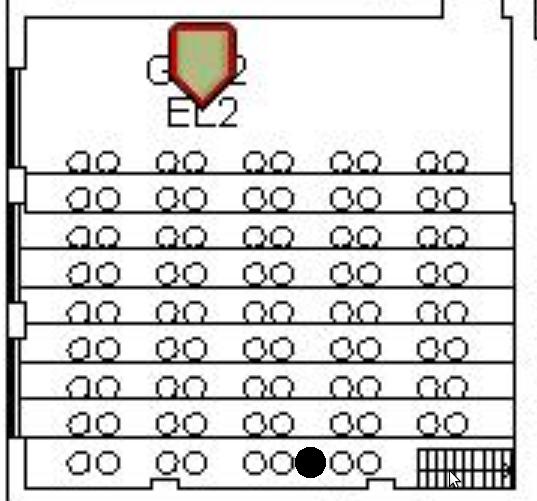
\includegraphics[width=5cm,keepaspectratio=true]{back}\\
\multicolumn{2}{|c|}{measurement at the backside}\\
\hline
\end{tabular}
\caption{microphone positions}
\label{tab:revmeasure}
\end{center}
\end{table}
\subsubsection{Results}
The reverbation time was analyzed with WinLMS and an average has been calculated with
$$T_{60,avg}=\frac{T_{60,front}+T_{60,middle}+T_{60,back}}{3}$$
The values for the reverbation times and the averages are listed in table \ref{tab:Tmeasurements}. Here one special result can be obtained. The reverbation time for the octave band $125Hz$ is much longer than for the other octave bands. One further measurement result is worth mentioning. At the front corner the reverbation time at $250Hz$ is very low. This can be caused due to negative interference at the microphone position. The measurement results from WinLMS are listed in figures \ref{fig:reverbationfront}, \ref{fig:reverbationmiddle} and \ref{fig:reverbationback}. The plots show that at low frequencies the reverbation times differ very much. This is because of the large wavelength. The amplitudes at the microphones differ very much, so the reverbation times differ much too. Generally it can be obtained that the reverbation times are decreasing slightly with increasing frequency.
\begin{table}
\begin{center}
\begin{tabular}{|c||c|c|c||c|}
\hline
octave band & back & middle & front & average	\\
$Hz$		&	$s$	&	$s$		&	$s$		&	$s$		\\
\hline
\hline
125			& 1.34	&	0.98	&	1.58	&	1.3		\\
\hline
250			& 0.86	&	0.72	&	0.07	&	0.55	\\
\hline
500			& 0.75	& 	0.78	&	0.49	&	0.67	\\
\hline
1k			& 0.73	&	0.72	&	0.72	&	0.72	\\
\hline
2k			& 0.75	&	0.78	&	0.78	&	0.77	\\
\hline
4k			& 0.64	&	0.63	&	0.65	& 	0.64	\\
\hline
\end{tabular}
\caption{$T_{60}$ measurements and average}
\label{tab:Tmeasurements}
\end{center}
\end{table}
\begin{figure}[htbp]
\begin{center}
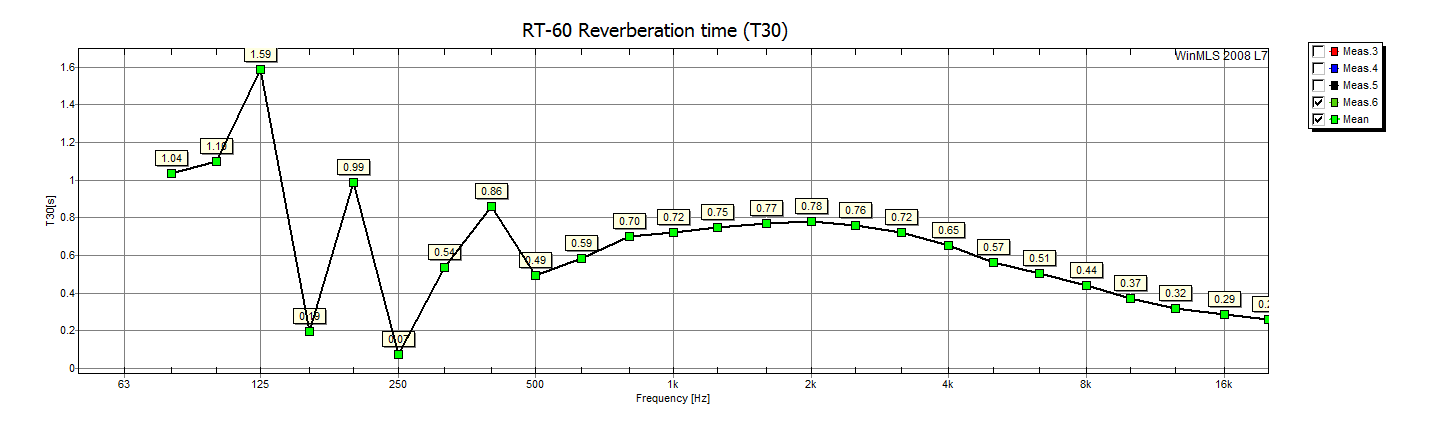
\includegraphics[width=15cm,keepaspectratio=true]{reverbationfront}
\caption{reverbation time in the front position}
\label{fig:reverbationfront}
\end{center}
\end{figure}
\begin{figure}[htbp]
\begin{center}
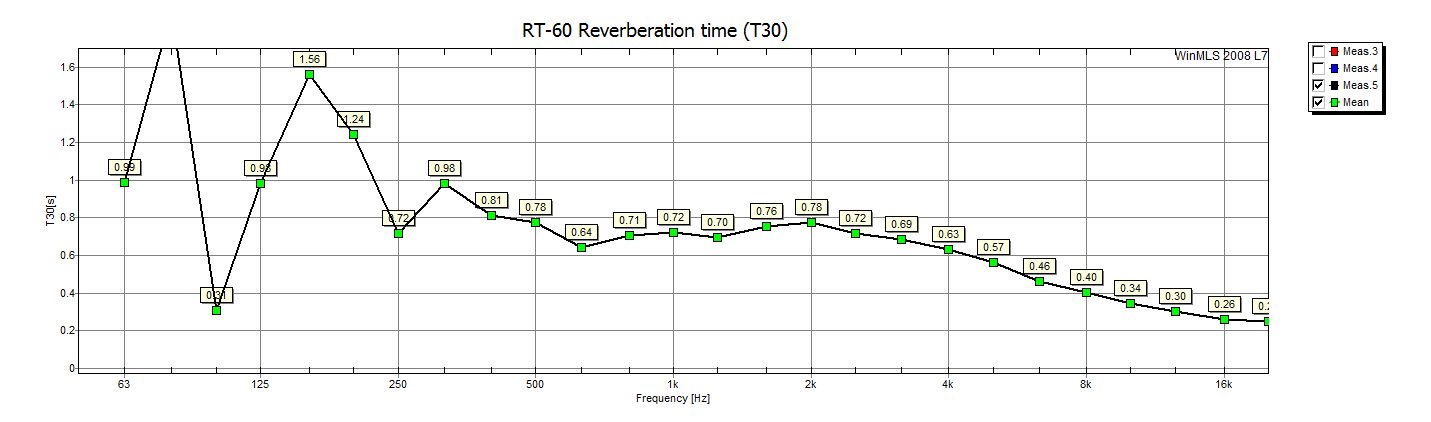
\includegraphics[width=15cm,keepaspectratio=true]{reverbationmiddle}
\caption{reverbation time in the middle position}
\label{fig:reverbationmiddle}
\end{center}
\end{figure}
\begin{figure}[htbp]
\begin{center}
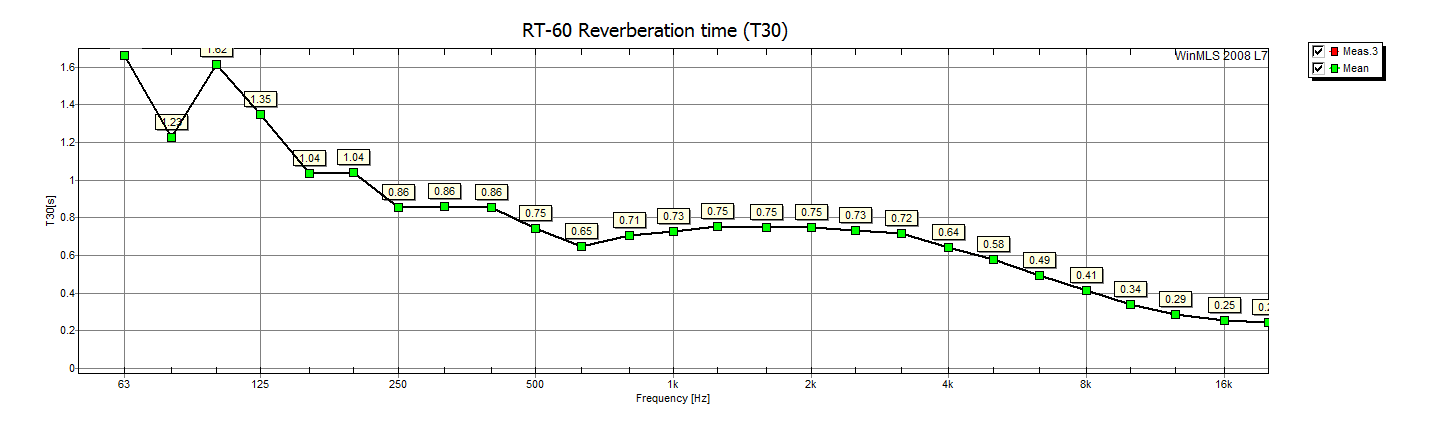
\includegraphics[width=15cm,keepaspectratio=true]{reverbationback}
\caption{reverbation time in the back position}
\label{fig:reverbationback}
\end{center}
\end{figure}
\subsection{Sound pressure level}
\subsubsection{Method}
For measuring the sound pressure level as function of distance the sound presure level of pink noise was measured in different distances from the sound source. The SPL of the 500Hz-band was calculated by using WinLMS. The measurements were started at shortest distance to the sound source, and further measurements were done in increasing distance. Between measurements points are about 0.25m to 1m of distance. 
\subsubsection{Results}
The measured results are put into Matlab and plotted as function over distance and listed in figure \ref{fig:spl}. Here it can be obtained that the sound pressure level is decreasing until the critical distance (hall radius) is reached. After this the decrease is much slower due to strong interferences with reverbation.
\begin{figure}[htbp]
\begin{center}
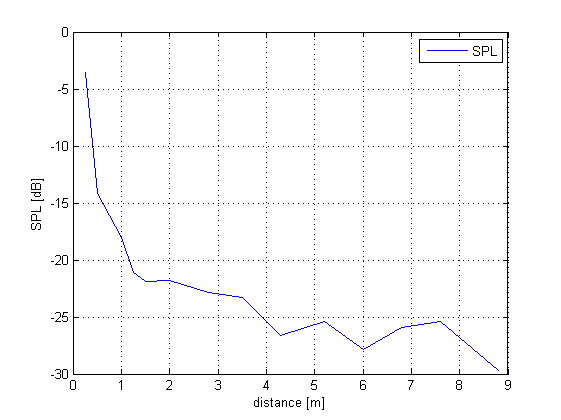
\includegraphics[width=10cm,keepaspectratio=true]{SPL}
\caption{Sound Pressure Level as function of distance}
\label{fig:spl}
\end{center}
\end{figure}

\newpage
\section{Calculations}
\subsection{absorbtion coefficients}
The absorbtion coefficients for each band are calculated according to Sabine's formula. The values $T_{60}$ which are used are the average values of the measured results. 
$$\bar{\alpha_{125}}=\frac{0.161\cdot 367m^3}{1.3s\cdot 344m^2}=0.132$$
$$\bar{\alpha_{250}}=\frac{0.161\cdot 367m^3}{0.55s\cdot 344m^2}=0.312$$
$$\bar{\alpha_{500}}=\frac{0.161\cdot 367m^3}{0.67s\cdot 344m^2}=0.256$$
$$\bar{\alpha_{1k}}=\frac{0.161\cdot 367m^3}{0.72s\cdot 344m^2}=0.239$$
$$\bar{\alpha_{2k}}=\frac{0.161\cdot 367m^3}{0.77s\cdot 344m^2}=0.223$$
$$\bar{\alpha_{4k}}=\frac{0.161\cdot 367m^3}{0.64s\cdot 344m^2}=0.268$$

\subsection{absorbtion with chair surfaces}
$$\alpha_{1,125}=\frac{344m^2\cdot 0.132-0.7\cdot 66.75m^2}{277.25m^2}=-0.004$$
The absorbtion factor is negative which means that the chair absorption factor is overestimated. Due to the fact that absorbtion decreases with lower frequencies the absorption factor is lower at low frequencies.  An factor of $\alpha=0.4$ for a frequency of $f=125Hz$ was assumed and the resulting absorbtion factor increases to
 $$\alpha_{1,125}=\frac{344m^2\cdot 0.132-0.4\cdot 66.75m^2}{277.25m^2}=-0.067$$
All other calculations are done with an assumed absorbtion factor of $\alpha_{chair}=0.7$.
 $$\alpha_{1,250}=\frac{344m^2\cdot 0.312-0.7\cdot 66.75m^2}{277.25m^2}=0.219$$
 $$\alpha_{1,500}=\frac{344m^2\cdot 0.256-0.7\cdot 66.75m^2}{277.25m^2}=0.149$$
 $$\alpha_{1,1k}=\frac{344m^2\cdot 0.239-0.7\cdot 66.75m^2}{277.25m^2}=0.128$$
 $$\alpha_{1,2k}=\frac{344m^2\cdot 0.223-0.7\cdot 66.75m^2}{277.25m^2}=0.108$$
 $$\alpha_{1,4k}=\frac{344m^2\cdot 0.268-0.7\cdot 66.75m^2}{277.25m^2}=0.164$$

\subsection{absorption material}
$$\bar{\alpha}=\frac{0.161\cdot 367m^3}{344m^2\cdot 0.5s}=0.344$$
The materials given for this task are available for absorbtion factors $\alpha=0.3 ... 0.9$. The calculated vvalue of $\bar{\alpha}$ is in this range, so a absorber material with an average of $0.344$ can be used.

\subsection{hall radius}
The average reverbation time calculated as result of the three measurements was $T_{60,500}=0.67s$. The hall distance can be calculated with 
$$r_H=0.057\cdot\sqrt{\frac{V}{T_{60}}}=0.057\cdot\sqrt{\frac{367m^3}{0.67s}}=1.334m$$
Compared to the measured result it can be obtained that the calculated value is a little bit smaller than the measured one, which is about 1.5m. This is because for the calculation an omnidirectional sound soure was assumed. Due to the fact that the used loudspeaker is not omnidirectional but directed, the measured value is a little bit farer away from the sound source. 

\newpage
\section{Conclusion}
The topic of room acoustics was covered in the lab exercise. Room dimensions were measured with a laser meter and room attributes like volume and wall area were calculated. The chosen room EL2 in Elbygget had a nearly quadratical shape, a slope with chairs as main absorbtion material is inside. Further the reverbation time of the room in three different positions was measured in each octave band. As microphone positions one in the back, one in the middle and one in the front corner of the room were used. The points were chosen because of typical listening points in the auditorium as well as speaking position for the front point. Concerning the measured results it can be obtained that reverbation times are decreasing with increasing frequency. At low frequencies large differences between measured results can be seen due to large wavelength compared to the membrane size of the microphone.\\
The sound pressure level was measured as function of distance from the sound source. At this measurement it can be seen that sound pressure levels are decreasing rapidly until the hall radius is reached. The sound pressure levels decrease much slower below the critical distance point.\\
The average absorption factors of the lecture hall were calculated. It can be obtained that they mainly remain at a value of about 0.25 for the whole measured frequency range. The only different value is at 125Hz, where the absorption coefficient has a much lower value of 0.132. This is because of the larger measured reverbation time at low frequencies. Using Sabine's formula and an assumed absorption factor of 0.7 for the chair slope surface it can be seen, that the absorption coefficients for the remaining surfaces are getting lower, because of a quite high absorption factor of the chairs. At a frequency band of 125Hz the calculated value for absorption of the remaining surfaces got negative, which means that the absorption of the chair surface was overestimated. Due to a lower absorption factor at low frequencies, which is usually the case, an absorption factor of 0.4 for the chair surface at a frequency of 125Hz was assumed.\\
To get a lower reverbation time\footnote{It was required to lower down the reverbation time to 0.5s at 1kHz} Sabine's formula was modified. The average absorption factor of the room was calculated to a value of 0.344. Absorber materials were assumed to be available with absorption factors between 0.3 and 0.9, so that no further steps were required to lower down the reverbation time.\\
In a further step the hall radius was calculated. The sound source was assumed as omnidirectional. The calculated distance was at about 1.33m. As the measurements showed, the real hall radius was a little bit farer away due to non-omnidirectionality of the loudspeaker.
\newpage
\section{Appendix}
\subsection{Example calculations}

\subsubsection{Reverbation time in an auditorium}
\paragraph{geometric calculations}
$$V=12m\cdot 6m\cdot 15m - \frac{11m\cdot 12m\cdot 3m}{2}$$
$$V=882m^3$$

$$l_{slope}=\sqrt{(11m)^2+(3m)^2}=11.4m$$
$$S=12m\cdot 6m+2\cdot 15m\cdot 6m+3m\cdot 12m-2\cdot\frac{3m\cdot 11m}{2}+12m\cdot 15m+12m\cdot 4m+11.4m\cdot 12m$$
$$S=619.8m^2$$

\paragraph{a) calculation of $\alpha$}
$$\bar{\alpha}=\frac{0.161\cdot 882m^3}{619.8m^2\cdot 1s}$$
$$\alpha=0.229$$

\paragraph{b) calculation of absorption factor where the chairs are}
$$\alpha=\frac{0.229\cdot 619.8m^2-0.1\cdot 483m^2}{136.8m^2}$$
$$\alpha=0.684$$
\paragraph{c) hall radius}
$$r_H=\sqrt{\frac{882}{1s\cdot 100\cdot \pi}}=1.68m$$
\subsection{More accurate}

\paragraph{$f=2kHz$}
$$\bar{\alpha}=\frac{0.161\cdot 882m^3-483m^2\cdot 0.229-4\cdot \frac{0.074}{0.5}\cdot 2^2\cdot 882m^3}{136.8m^2}$$
$$\bar{\alpha}=$$
\paragraph{$f=4kHz$}
$$\bar{\alpha}=\frac{0.161\cdot 882m^3-483m^2\cdot 0.229-4\cdot \frac{0.074}{0.5}\cdot 4^2\cdot 882m^3}{136.8m^2}$$
$$\bar{\alpha}=$$
\subsection{Calculation of room parameters\label{sec:roomparam}}
\subsubsection{room volume}
The room volume can be calculated by calculating the room as whole cuboid and subtracting the volume below the slope.
\begin{equation}
V=V_{total}-V_{below\,slope}
\end{equation}
$$V=10m\cdot 4m\cdot 10m-\frac{6.6m\cdot 1m\cdot 10m}{2}$$
$$V=367m^3$$
\subsubsection{surface area}
\begin{equation}
S=S_{ceiling}+S_{floor}+S_{slope}+S_{front}+S_{back}+2\cdot S_{wall}
\end{equation}
$S_{ceiling}$ covers whole area above the lecture room, $S_{floor}$ defines the horizontal floor area. $S_{slope}$ covers all area on the slope, mainly the area where the chairs are in the room. The wall surface $S_{wall}$ is everything on the left and right side of the lecture hall. At this area the surface area below the slope has to be subtracted. $S_{front}$ and $S_{back}$ cover the front and the back part of the wall.\\
So the total surface area is
$$S=10m\cdot\sqrt{6.6^2m^2+1^2m^2}+3.4m\cdot 10m+10m\cdot 10m+10m\cdot 4m+10m\cdot 3m+2\cdot(\frac{4m\cdot 10m-6.6m\cdot 1m}{2})$$
$$S=344m^2$$
\newpage
\section{References}



\end{document}
